\documentclass[11pt,a4paper]{article}
\usepackage[margin=2.4cm]{geometry}
\usepackage{amsmath,amssymb,bm}
\usepackage{graphicx}
\usepackage{booktabs}
\usepackage{xcolor}
\usepackage[colorlinks=true,linkcolor=blue!60!black,citecolor=blue!60!black]{hyperref}
\usepackage{caption}
\captionsetup{font=small,labelfont=bf}

\newcommand{\uu}{\bm{u}}
\newcommand{\nn}{\bm{n}}
\newcommand{\tang}{\bm{t}}
\newcommand{\Sf}{\bm{S}_f}
\newcommand{\rAU}{r_{A_U}}
\newcommand{\rAtU}{r_{A_tU}}

\title{\bf Free-slip immersed boundaries for a collocated SIMPLEC solver\\
\large Two routes: ghost extrapolation and partial face areas}
\author{Notes generated during solver development}
\date{\today}

\begin{document}
\maketitle

\begin{abstract}
We extend the implicit second-order immersed-boundary method of Luchini, Gatti, Chiarini,
Gattere, Atzori \& Quadrio (\emph{J.\ Comput.\ Phys.}\ \textbf{539} (2025) 114245) from
no-slip to \emph{free-slip} boundaries, inside a collocated finite-volume SIMPLEC solver.
The original method folds the entire boundary correction into the centre weight of the
Laplacian stencil. We show that free slip is obtained by replacing the Dirichlet wall value
with the \emph{tangential projection} of the first fluid point, which keeps the correction in
the same place but introduces a coupling between the velocity components. We then document
three distinct $O(1)$ errors that appear if the construction is applied only partially, and
two instabilities that appear if it is applied naively, together with the measurements that
identify each. The final scheme reproduces uniform flow along an oblique free-slip wall to
$2\times10^{-6}$ where the staircase alternative is wrong by $1.2\times10^{-1}$, and runs at
every resolution tested on both a coupled and a segregated momentum route.

We then present a second, independent route based on \emph{partial face areas} (cut cells).
There the boundary condition is carried entirely by a geometric closure identity, so no ghost
value, no blanking and no cross term are needed at all. It reproduces the oblique-wall test
exactly ($g_x=0$ to the last bit) and makes the discrete continuity error machine-zero in both
the fluid and the solid, which the ghost route does not achieve. We document both, and say
plainly which to prefer and why.
\end{abstract}

\tableofcontents

\part*{Part I --- The ghost-extrapolation route}
\addcontentsline{toc}{section}{Part I --- The ghost-extrapolation route}

\section{Governing equations and baseline discretisation}

We solve the incompressible Navier--Stokes equations
\begin{equation}
\frac{\partial \uu}{\partial t}+\nabla\!\cdot\!(\uu\uu)-\nabla\!\cdot\!(\nu\nabla\uu)
=-\nabla p+\bm{g},\qquad \nabla\!\cdot\!\uu=0,
\end{equation}
with $p$ the reduced pressure, on a uniform doubly periodic Cartesian grid. The
discretisation is cell-centred (collocated): $u$, $v$ and $p$ all live at cell centres, and
the five-point stencil is stored as five coefficient arrays rather than as a matrix. Time
advance is implicit Euler used as pseudo-transient continuation, and the pressure--velocity
coupling is SIMPLEC exactly as in OpenFOAM's \texttt{simpleFoam}:
\begin{align}
a_P\uu_P &= H(\uu)-V\nabla p, & H(\uu)&=b-\textstyle\sum_{nb}a_{nb}\uu_{nb},\\
\rAU&=1/a_P, & \rAtU&=1/\Big(a_P+\textstyle\sum_{nb}a_{nb}\Big),\\
\nabla\!\cdot\!\big(\rAtU V\nabla p\big)&=\nabla\!\cdot\!\phi_{HbyA}, &
\phi&=\phi_{HbyA}-\rAtU V\,\mathrm{snGrad}(p)|\Sf|.
\end{align}

\subsection{Constant flow rate}
Free slip generates no friction, so a fixed body force gives no steady state: the flow
accelerates without bound. We therefore fix the bulk velocity and let the force follow.
Because only the source term depends on $g_x$, and one predictor--projection pass is
\emph{affine} in it, two passes --- one at $g_x=0$ and one at $g_x=1$ --- give the exact
$g_x$ that lands the bulk velocity on its target:
\begin{equation}
g_x=\frac{U_b^{\rm target}-U_b^{(0)}}{U_b^{(1)}-U_b^{(0)}} .
\end{equation}
There is no gain to tune and both passes share the matrix factorisations. A proportional
controller was tried first and diverged, because free slip leaves the bulk mode almost
undamped.

\section{The no-slip starting point}

For no slip, Eq.~(6) of Luchini \emph{et al.} replaces the ghost value at the first point
inside the solid by a linear extrapolation between the first fluid point and the wall,
\begin{equation}
u_{\rm ghost}=\Big(1-\frac{h}{\delta}\Big)u_P ,
\label{eq:eq6}
\end{equation}
with $h$ the mesh spacing and $\delta$ the distance from the cell centre to the wall along
that stencil arm (Fig.~\ref{fig:sketch}). Substituting back into the Laplacian moves the
whole correction into the \emph{centre} weight, so nothing is stored at the ghost point and
corrections from different directions are additive. Crucially the correction \emph{increases}
diagonal dominance as $\delta\to0$, which is what makes the method robust.

\begin{figure}[t]\centering
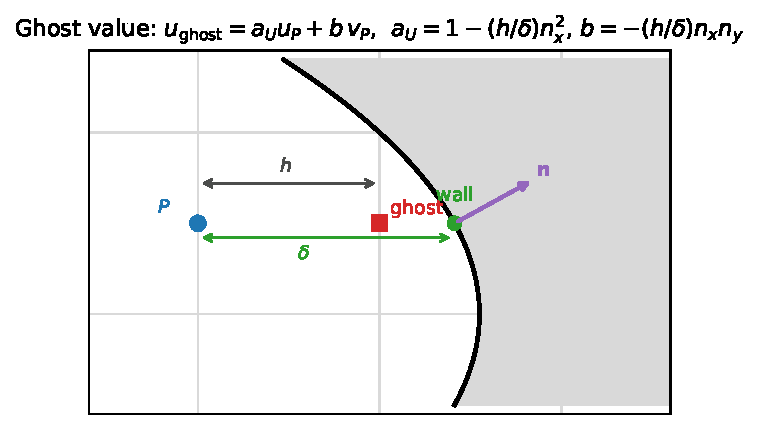
\includegraphics[width=0.62\textwidth]{figs/ghost_sketch.pdf}
\caption{Ghost construction on a cut stencil arm. $P$ is the first fluid point, $\delta$ the
distance to the true boundary, $h$ the mesh spacing, $\nn$ the local surface normal. For no
slip the wall value is zero; for free slip it is the tangential projection of $\uu_P$.}
\label{fig:sketch}
\end{figure}

\section{Free slip: the tangential projection}

Free slip means no penetration \emph{and} zero tangential gradient. The second condition says
the tangential velocity does not change along the normal, so to leading order the wall
velocity equals the tangential part of the first fluid point:
\begin{equation}
\uu_{\rm wall}=(I-\nn\nn^{T})\,\uu_P ,
\label{eq:proj}
\end{equation}
which is precisely the single scalar constraint $\uu_{\rm wall}\!\cdot\!\nn=0$ written out.
Feeding \eqref{eq:proj} through the same linear extrapolation that produced \eqref{eq:eq6}
gives, for the $x$-momentum,
\begin{equation}
\boxed{\;u_{\rm ghost}=a_U\,u_P+b\,v_P,\qquad
a_U=1-\frac{h}{\delta}n_x^{2},\qquad b=-\frac{h}{\delta}n_xn_y\;}
\label{eq:ghost}
\end{equation}
and symmetrically $a_V=1-(h/\delta)n_y^{2}$ for the $y$-momentum. Setting the projector to
the identity ($n_x^2\to1$, $n_xn_y\to0$) recovers \eqref{eq:eq6} exactly; we verified that the
resulting stencil coefficients are bitwise identical to the no-slip ones.

So the centre weight picks up $n_x^{2}$ in place of $1$, and a \textbf{cross term} appears in
the other component. Everything else about the method is preserved: one value per cut arm, no
stored ghosts, additive across directions.

\subsection{Why a single constraint per cell matters}
An earlier version imposed no penetration once per cut \emph{arm}: $u=0$ on $x$-arms and
$v=0$ on $y$-arms. On a curved boundary a cell can have both an $x$- and a $y$-arm cut, and
both components are then pinned --- the cell becomes a no-slip patch. Measured over five
grids, the surface slip velocity decayed as $|u_t|\propto\Delta$: the scheme converged to
\emph{no slip}. Equation~\eqref{eq:proj} removes this, because a cell whose normal is mostly
along $y$ gets $n_x^{2}\approx0$ on its $x$-arm too, leaving $u$ free.

\section{Three places the ghost must be used}

The ghost is not a Laplacian-only correction. Free slip fails, each time at $O(1)$, if it is
omitted from any of three places.

\paragraph{(i) The viscous stencil.} As derived above.

\paragraph{(ii) The face fluxes.} Closing cut faces on the staircase (a boolean mask) blocks
the tangential flux, because for an oblique wall the tangential velocity has a component
normal to every axis face. Using the ghost instead, a uniform tangential field gives
$u_{\rm ghost}=u_P$ --- the projector is the identity on such a field --- so every one of a
cut cell's four \emph{full} faces carries the uniform flux and the discrete divergence is
identically zero. Measured on a $45^\circ$ wall: $\max|\nabla\!\cdot\!\phi|$ over fluid cells
is $1.2\times10^{-1}$ with masks and $4.4\times10^{-10}$ with the ghost.

\paragraph{(iii) The convective stencil.} The original paper notes that no correction of the
convective terms is needed for second order. That is true \emph{for no slip}, where $u_P\to0$
at the wall makes the term negligible. Under free slip $u_P$ is $O(U)$, and reading the
blanked zero out of the solid neighbour is an $O(1)$ error. Section~\ref{sec:evidence}
quantifies it.

\section{Two instabilities, and their cure}

\subsection{The cross term must not be indefinite}
Collecting the ghost contributions, each cut arm adds to the local $2\times2$ block
\begin{equation}
\frac{h}{\delta}\,\nn\nn^{T}\times
\begin{cases}
+\nu & \text{(viscous)}\\[2pt]
\tfrac12 f & \text{(convective, central)}
\end{cases}
\end{equation}
where $f$ is the face volume flux. Since $\nn\nn^{T}$ is rank-one positive semi-definite, the
viscous block is $a_PI+\nu\frac{h}{\delta}\nn\nn^{T}$, with eigenvalues $a_P+\nu h/\delta$
along $\nn$ and $a_P$ along $\tang$: well posed, constrained in the normal direction only ---
which is exactly what free slip means --- and increasingly dominant as $\delta\to0$
(Fig.~\ref{fig:spec}, left). The convective copy carries $f$, which \emph{changes sign}, so
that block is indefinite (Fig.~\ref{fig:spec}, right). Making an indefinite block implicit
does not make it well posed: a central convective ghost diverged whether it was lagged,
lagged with a diagonal repair, clipped in $h/\delta$, or solved fully implicitly.

\begin{figure}[t]\centering
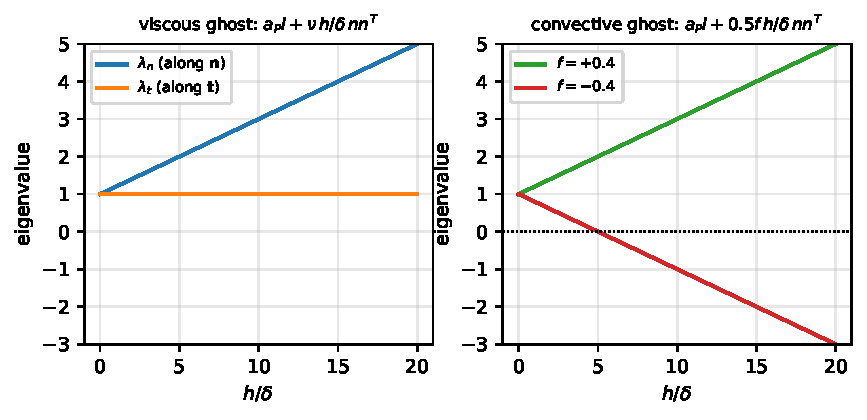
\includegraphics[width=0.92\textwidth]{figs/block_spectrum.pdf}
\caption{Eigenvalues of the local $2\times2$ momentum block against $h/\delta$. Left: the
viscous ghost is positive semi-definite and stabilising. Right: the convective ghost carries
the face flux $f$, and for $f<0$ the block loses positivity.}
\label{fig:spec}
\end{figure}

\paragraph{Cure: upwind the cut arms.} The ghost is a \emph{neighbour} value, so it should
only be picked up on inflow faces. With upwinding the inflow contribution becomes
\begin{equation}
f\Big(I-\frac{h}{\delta}\nn\nn^{T}\Big)=-|f|I+|f|\frac{h}{\delta}\nn\nn^{T},\qquad f<0,
\end{equation}
whose rank-one part is positive semi-definite again, while the $-|f|I$ part is balanced by
$+f$ on the outflow faces exactly as in ordinary upwinding. Uniform flow parallel to the wall
remains exact, because upwind and central agree for a constant field. Only cut arms are
upwinded; the scheme stays central everywhere else.

\subsection{The remaining positivity defect, and the S1/S3 stabilisation}
Upwinding is not quite sufficient. On a cut arm the inflow term has \emph{no off-diagonal to
land on} --- the neighbour is solid --- so it falls on the diagonal, and on a few cells very
close to the wall it pushes the diagonal non-positive. At $n_x=41$ this happened on two cells,
which drove $\rAtU$ to $-121$, turned the pressure Laplacian indefinite, and produced an
exactly singular factorisation. The distribution of $\delta/h$ (Fig.~\ref{fig:delta}) explains
why $n_x=41$ is the outlier: its closest cut cell sits at $\delta/h=0.024$ against $0.151$ at
$n_x=81$ --- a geometric lottery, not a resolution trend.

\begin{figure}[t]\centering
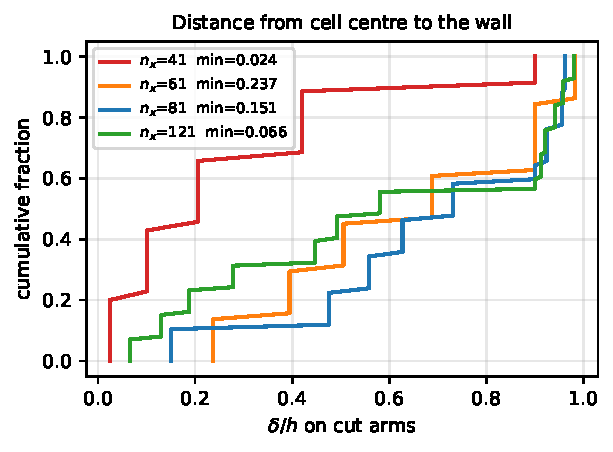
\includegraphics[width=0.52\textwidth]{figs/delta_distribution.pdf}
\caption{Cumulative distribution of $\delta/h$ over cut arms for the circular cylinder. The
minimum is a geometric accident of how the circle meets the grid, which is why $n_x=41$ fails
first rather than the coarsest or finest mesh.}
\label{fig:delta}
\end{figure}

\paragraph{S1 --- floor the SIMPLEC mobilities.} $\rAU$ and $\rAtU$ are floored at $V/\Delta t$,
the value an unobstructed cell would have, so the pressure Laplacian cannot turn indefinite.
This is necessary but not sufficient: with S1 alone the failure changes from a singular
factorisation to divergence.

\paragraph{S2 --- a global P\'eclet blend (rejected).} Weighting the ghost by
$\min(1,C\nu/|f|)$ does restore convergence at every resolution, but it gives up consistency
\emph{everywhere} the blend is active in order to rescue a handful of cells: the coarse-grid
drag moved by $20\%$ as the constant $C$ was varied over a decade. We report it because it
works, and discard it because S3 is strictly better.

\paragraph{S3 --- an adaptive per-cell blend (adopted).} On each cut cell we take
\begin{equation}
\text{contribution}=w\,(\text{ghost, upwinded})+(1-w)\,(\text{plain central}),
\end{equation}
with $w\in[0,1]$ the largest value that keeps the momentum diagonal at or above a floor. The
diagonal is linear in $w$, so $w$ follows in closed form and no iteration is needed. Cells
that do not need help keep $w=1$ and remain fully consistent. At $n_x=41$ the blend engages on
\textbf{2 of 1216 fluid cells} (Fig.~\ref{fig:s3}) --- precisely the two diagnosed above.

\begin{figure}[t]\centering
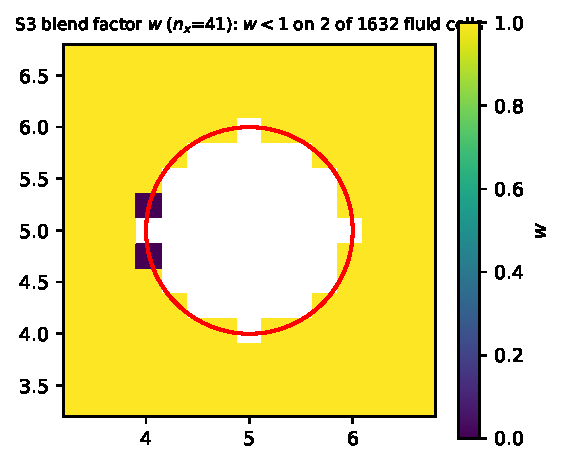
\includegraphics[width=0.48\textwidth]{figs/s3_activation.pdf}
\caption{The S3 blend factor $w$ at $n_x=41$. $w=1$ (full ghost, fully consistent) everywhere
except two cells adjacent to the wall.}
\label{fig:s3}
\end{figure}

\section{Coupled versus segregated momentum, and a Rhie--Chow trap}

The cross term couples $u$ and $v$ at the \emph{same} cell only, so the coupled block matrix
\begin{equation}
\begin{bmatrix} A_{uu} & \mathrm{diag}(c_U)\\ \mathrm{diag}(c_V) & A_{vv}\end{bmatrix}
\begin{bmatrix}u\\v\end{bmatrix}=\begin{bmatrix}b_u\\b_v\end{bmatrix}
\end{equation}
has six nonzeros per row instead of five --- far cheaper than a general block-coupled solve.
$H(\uu)$ then carries the cross contribution, exactly as OpenFOAM's \texttt{H()} does.

The segregated alternative lags the cross term and adds $|c|$ to the diagonal to keep the
lagged iteration diagonally dominant, subtracting it again on the right with the lagged value
of the same component so that the fixed point is unchanged. \textbf{This repair is not free.}
It inflates $a_P$, which changes $\rAU$ and $\rAtU$, and hence the Rhie--Chow flux --- a
different but self-consistent pressure--velocity coupling. Removing the repair makes the two
routes agree exactly (Table~\ref{tab:rc}). Note also that $a_P$ \emph{must} be the repaired
diagonal: $H(\uu)/a_P$ telescopes to $\uu+\rAU\nabla p$ only if $a_P$ is the diagonal the
predictor actually solved with. Using the unrepaired one breaks the identity and produced a
negative drag in our tests.

\begin{table}[h]\centering
\caption{Effect of the segregated diagonal repair, $\nu=0.4$, $n_x=61$.}
\label{tab:rc}
\begin{tabular}{lcc}
\toprule
 & drag & field difference vs coupled\\
\midrule
coupled                      & 1.251539 & ---\\
segregated, repair removed   & 1.251539 & $4.0\times10^{-6}$\\
segregated, with repair      & 1.256236 & $4.6\times10^{-3}$\\
\bottomrule
\end{tabular}
\end{table}

\section{Numerical evidence}\label{sec:evidence}

\subsection{Uniform flow along an oblique free-slip wall}
The sharpest test available: a free-slip channel at $45^\circ$ to the grid, driven at fixed
flow rate. The exact solution is uniform flow parallel to the walls with \emph{zero} driving
force. Table~\ref{tab:w45} gives the result with and without the convective ghost.

\begin{table}[h]\centering
\caption{$45^\circ$ free-slip channel, $\nu=0.4$. Exact answer: $\max u-\min u=0$ and
$g_x=0$. All cases converged to a residual of $10^{-9}$.}
\label{tab:w45}
\begin{tabular}{llcccc}
\toprule
 & & \multicolumn{2}{c}{ghost on} & \multicolumn{2}{c}{ghost off}\\
\cmidrule(lr){3-4}\cmidrule(lr){5-6}
route & $n_x$ & $\max u-\min u$ & $g_x$ & $\max u-\min u$ & $g_x$\\
\midrule
coupled     & 41 & $1.9\times10^{-6}$ & $-4.9\times10^{-9}$ & $1.232\times10^{-1}$ & $2.18\times10^{-3}$\\
coupled     & 81 & $3.4\times10^{-6}$ & $-1.0\times10^{-8}$ & $1.024\times10^{-1}$ & $2.04\times10^{-3}$\\
segregated  & 41 & $2.2\times10^{-6}$ & $-2.2\times10^{-8}$ & $1.211\times10^{-1}$ & $2.07\times10^{-3}$\\
segregated  & 81 & $3.4\times10^{-6}$ & $-6.3\times10^{-8}$ & $9.959\times10^{-2}$ & $1.98\times10^{-3}$\\
coupled     & 161 & $2.9\times10^{-6}$ & $-6.8\times10^{-9}$ & $8.307\times10^{-2}$ & $1.77\times10^{-3}$\\
segregated  & 161 & $3.7\times10^{-6}$ & $-8.3\times10^{-8}$ & $8.127\times10^{-2}$ & $1.70\times10^{-3}$\\
\bottomrule
\end{tabular}
\end{table}

The ghost-off error is not merely large, it is \textbf{h-independent}: halving $\Delta$ moves
it by a factor $1.2$. Over two successive refinements ($41\to81\to161$) the observed order of
the velocity spread is $0.27$ then $0.30$, and that of the spurious drag $0.09$ then $0.21$
(Fig.~\ref{fig:w45}) --- flat, not converging. A grid-refinement study therefore shows a tidy convergent
sequence --- onto the wrong answer. This is the central argument for carrying the ghost into
the convective term.

\begin{figure}[t]\centering
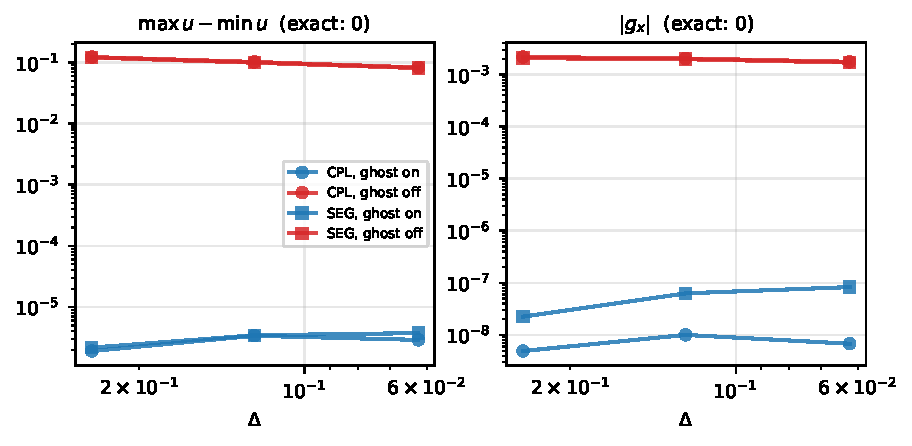
\includegraphics[width=0.92\textwidth]{figs/wall45_error.pdf}
\caption{Error on the $45^\circ$ free-slip channel against mesh spacing. With the ghost the
error sits at the solver tolerance; without it the error is essentially independent of
$\Delta$.}
\label{fig:w45}
\end{figure}

\subsection{Cylinder drag}
Table~\ref{tab:drag} gives the drag on a free-slip circular cylinder in a periodic box at
fixed flow rate, with the full scheme (upwind ghost, S1, S3), on both momentum routes. All
resolutions run stably on both routes.

\begin{table}[h]\centering
\caption{Free-slip cylinder, $Re_R=UR/\nu=1.25$, $\nu=0.4$, all converged to $10^{-9}$.
Drag is $g_xA_{\rm fluid}$, which balances the body force at steady state.}
\label{tab:drag}
\begin{tabular}{lcccc}
\toprule
$n_x$ & 41 & 61 & 81 & 121\\
$\Delta$ & 0.2439 & 0.1639 & 0.1235 & 0.0826\\
\midrule
coupled     & 1.236070 & 1.249283 & 1.247104 & 1.250610\\
segregated  & 1.263816 & 1.254353 & 1.250983 & 1.254389\\
\bottomrule
\end{tabular}
\end{table}

\begin{figure}[t]\centering
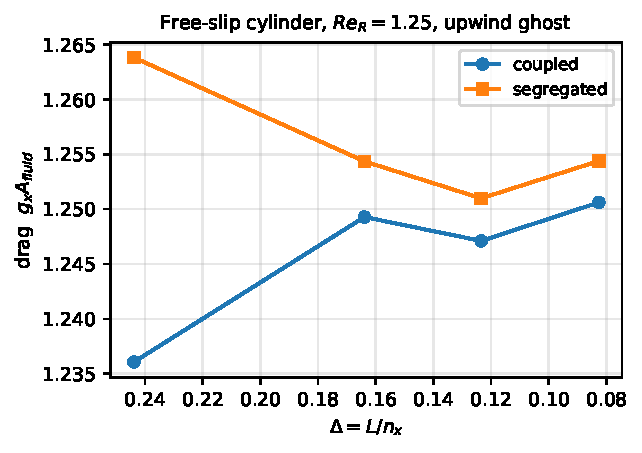
\includegraphics[width=0.52\textwidth]{figs/drag_convergence.pdf}
\caption{Cylinder drag against mesh spacing for both momentum routes.}
\label{fig:drag}
\end{figure}

\subsection{Stability coverage}
Table~\ref{tab:cov} records which combinations run. The central convective ghost fails widely;
upwinding repairs the segregated route outright and the coupled route down to $n_x=61$; adding
S1 and S3 closes the remaining case.

\begin{table}[h]\centering
\caption{Does the case reach a $10^{-9}$ residual? Cylinder, $\nu=0.1$, ghost on.}
\label{tab:cov}
\begin{tabular}{lccc}
\toprule
scheme & $n_x=41$ & $n_x=61$ & $n_x=81$\\
\midrule
central ghost, segregated        & no  & no  & yes\\
central ghost, coupled           & no  & no  & no \\
upwind ghost, segregated         & yes & yes & yes\\
upwind ghost, coupled            & no  & yes & yes\\
upwind ghost + S1 + S3, both     & yes & yes & yes\\
\bottomrule
\end{tabular}
\end{table}

\subsection{The flow field}
Figure~\ref{fig:field} shows the converged free-slip cylinder with and without the convective
ghost, and Fig.~\ref{fig:slip} the tangential slip velocity around the surface. Without the
ghost the near-wall velocity is visibly suppressed --- the boundary behaves partly as no slip,
which is the $O(1)$ error of Table~\ref{tab:w45} seen in physical space.

\begin{figure}[t]\centering
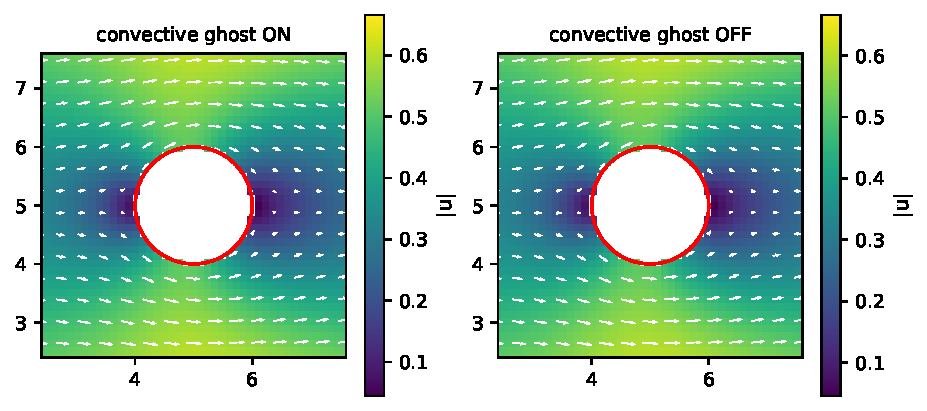
\includegraphics[width=0.86\textwidth]{figs/cylinder_field.pdf}
\caption{Velocity magnitude and vectors for the free-slip cylinder, $n_x=81$, $Re_R=1.25$.}
\label{fig:field}
\end{figure}

\begin{figure}[t]\centering
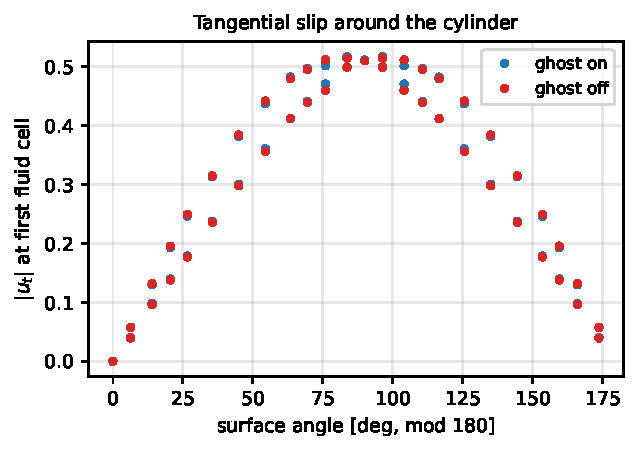
\includegraphics[width=0.56\textwidth]{figs/surface_slip.pdf}
\caption{Tangential velocity at the first fluid cell around the cylinder. The convective ghost
restores the slip that the blanked-neighbour treatment suppresses.}
\label{fig:slip}
\end{figure}


\part*{Part II --- The partial-face-area (cut-cell) route}
\addcontentsline{toc}{section}{Part II --- The partial-face-area route}

\section{Motivation}

The ghost route of Part~I leaves one defect: continuity is not machine-zero. Removing the
face masks makes the body transparent to tangential flow while its interior is still blanked
to $\uu=0$, so the ghost extension is discontinuous where it meets the blanked interior, and
the resulting divergence source in the first solid layer cannot be removed by the projection
because $\rAtU$ there is the blanking penalty. It also needs upwinding plus the S1/S3
stabilisation to survive at all resolutions.

Both problems have the same origin: a face is either fully open or fully closed. Giving each
face a \emph{fluid area fraction} removes it.

\section{Geometry}

Each face carries $\theta\in[0,1]$, the fraction of the face lying in the fluid, and each cell
carries $\alpha$, the fluid fraction of its volume. Both are obtained from the same level set:
$\theta$ by bisection along the face, $\alpha$ by sub-sampling. The fluid part of a cut cell is
a polygon bounded by the partially open axis faces and the wall segment
(Fig.~\ref{fig:cutcell}), and the two are tied together by
\begin{equation}
\sum_f \theta_f\,\nn_f A_f + \nn_{\rm wall}A_{\rm wall}=0 .
\label{eq:closure}
\end{equation}
Because $\theta$ and the wall segment come from the same level set, \eqref{eq:closure} holds
to machine precision. We verified it directly: on a straight oblique wall the normal recovered
from \eqref{eq:closure} matches the analytic normal to $2.2\times10^{-16}$, and a uniform field
parallel to that wall has \emph{exactly} zero discrete divergence.

\begin{figure}[t]\centering
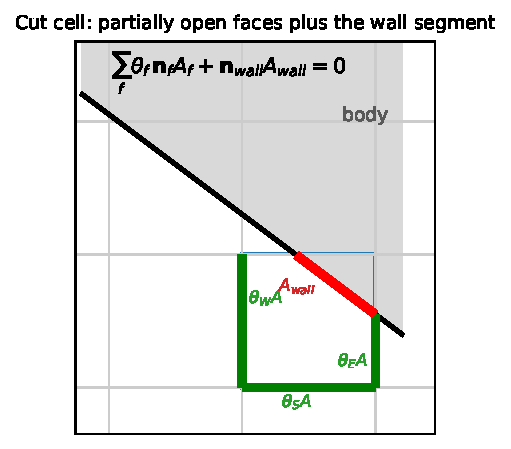
\includegraphics[width=0.52\textwidth]{figs/cutcell_sketch.pdf}
\caption{A cut cell. Its fluid boundary consists of the partially open axis faces (green) and
the wall segment (red); the two are linked by the closure identity \eqref{eq:closure}.}
\label{fig:cutcell}
\end{figure}

\section{The boundary condition falls out of the closure}

Equation~\eqref{eq:closure} carries the whole free-slip condition, term by term:

\begin{itemize}
\item \textbf{Viscous.} Free slip means zero tangential stress on the wall segment, and at
first order no normal viscous stress either, so the wall contributes nothing: the operator is
the $\theta$-weighted face sum, which annihilates a constant field.
\item \textbf{Convective.} No penetration means no flux through the wall segment, so again
only the $\theta$-weighted faces contribute.
\item \textbf{Pressure.} Here the wall \emph{does} contribute --- this is the form drag. With
$p_{\rm wall}=p_P$ to first order, \eqref{eq:closure} turns the Gauss gradient into
$\sum_f\theta_f(p_f-p_P)\nn_fA_f$, which vanishes for a uniform pressure, so no spurious force
is generated on a cut cell.
\item \textbf{Continuity.} $\sum_f\theta_f\phi_f=0$. Combined with \eqref{eq:closure}, a
uniform velocity in a cut cell satisfies this only if $\uu\!\cdot\!\nn_{\rm wall}=0$.
\end{itemize}

The last point deserves emphasis: \textbf{no penetration is never imposed anywhere. It emerges
from continuity plus closure.} Consequently this route has no ghost value, no blanking of cut
cells, no cross term between the velocity components, and needs none of the S1/S3
stabilisation of Part~I. Because the cross term is what distinguished the coupled from the
segregated momentum route, the two now produce \emph{bit-identical} results --- with no cross
coupling they solve the same block-diagonal system. We keep both files only so that the two
parts of this note have a matching pair each.

We verified each operator directly against the exact solution of the $45^\circ$ channel: the
viscous residual, the convective residual, the gradient of a uniform pressure and the
divergence of the exact field are all $0.000\times10^{0}$.

\section{Results}

\begin{table}[h]\centering
\caption{$45^\circ$ free-slip channel, $\nu=1$. Exact answer: uniform flow, $g_x=0$.}
\label{tab:cc45}
\begin{tabular}{lcc}
\toprule
 & ghost route & cut cells\\
\midrule
drag (exact $0$)                                   & $-4.9\times10^{-9}$ & $\bm{0.000000}$\\
mean $|\nabla\!\cdot\!\phi|$, fluid                & $4\times10^{-6}$    & $\bm{2\times10^{-18}}$\\
mean $|\nabla\!\cdot\!\phi|$, first solid layer    & $4.8\times10^{-3}$  & $\bm{0}$\\
\bottomrule
\end{tabular}
\end{table}

\begin{figure}[t]\centering
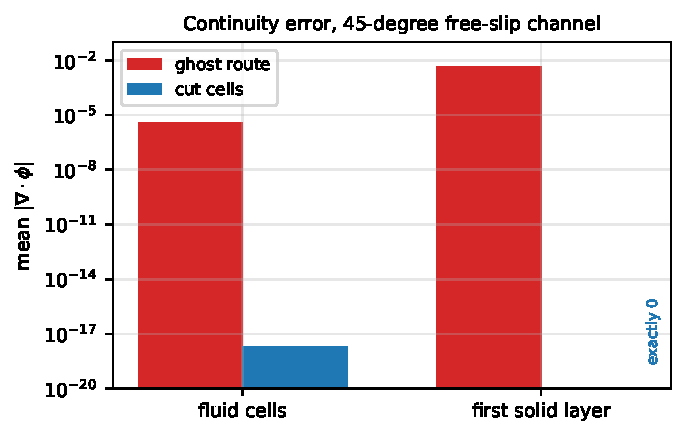
\includegraphics[width=0.52\textwidth]{figs/continuity_compare.pdf}
\caption{Discrete continuity error on the $45^\circ$ channel. The cut-cell route is exact in
both the fluid and the solid; the ghost route leaves a source in the first solid layer.}
\label{fig:cont}
\end{figure}

\begin{table}[h]\centering
\caption{Free-slip cylinder, cut-cell route. All cases converged to $10^{-9}$, symmetry held
to $10^{-14}$, continuity machine-zero. Coupled and segregated agree to the last digit.}
\label{tab:ccdrag}
\begin{tabular}{lcccc}
\toprule
$n_x$ & 41 & 61 & 81 & 121\\
\midrule
$\nu=1.0$ ($Re_R=0.5$) & 2.829667 & 2.907463 & 2.938772 & 2.977790\\
$\nu=0.5$ ($Re_R=1.0$) & 1.449213 & 1.487457 & 1.503127 & 1.523026\\
\bottomrule
\end{tabular}
\end{table}

\begin{figure}[t]\centering
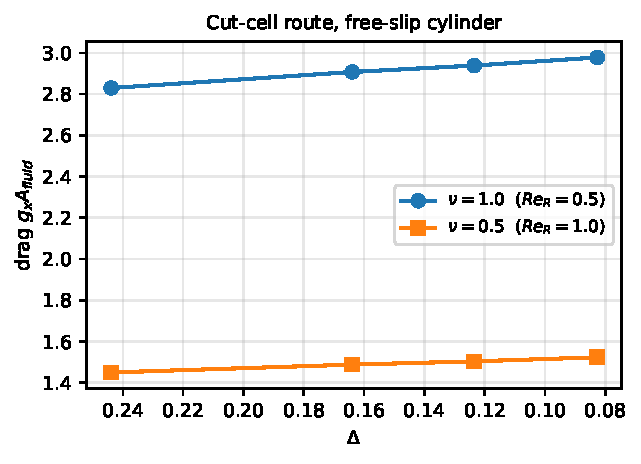
\includegraphics[width=0.52\textwidth]{figs/drag_cutcell.pdf}
\caption{Cut-cell drag against mesh spacing at the two viscosities.}
\label{fig:ccdrag}
\end{figure}

\section{The one cost: small cells}

Cut cells with $\alpha\to0$ have vanishing volume against $O(h)$ faces --- the classic
small-cell problem. We absorb slivers with $\alpha<\alpha_{\min}$ into the body. This is the
only place the route gives ground, and it has a trap: \textbf{an absorbed cell must have its
faces closed as well}, or the closure identity \eqref{eq:closure} is broken for its neighbours
and the exactness above is lost. We hit exactly this during development --- the divergence of
the exact field jumped from $0$ to $6\times10^{-2}$, i.e.\ $O(h)$, until the faces of absorbed
cells were zeroed too. Absorbing moves the boundary by $O(\alpha_{\min}h)$, which is within the
first-order error; cell merging would remove even that.

A second trap, worth recording because it is invisible until it is not: on a doubly periodic
grid the faces at $x=0$ and $x=L_x$ are the \emph{same} face. If $\theta$ is evaluated
independently at both, an inconsistent seam destroys conservation. We compute once and copy.
The same applies to the level set used for a test geometry: an oblique wall must be defined
through the periodic difference, or it does not close on the torus.

\section{Which route to use}

\begin{table}[h]\centering
\caption{The two routes compared.}
\label{tab:routes}
\begin{tabular}{lll}
\toprule
 & ghost (Part~I) & cut cells (Part~II)\\
\midrule
boundary condition   & imposed, via the ghost value      & emerges from closure\\
continuity           & $4\times10^{-6}$ fluid, $5\times10^{-3}$ solid & machine zero\\
oblique wall         & $\sim10^{-6}$                     & exact\\
extra machinery      & upwinding, S1, S3, cross term     & none\\
coupled vs segregated& differ (Rhie--Chow, Sec.~7)       & bit-identical\\
weak point           & positivity near the wall          & small cells\\
no-slip limit        & recovers Eq.~(6) exactly          & would need the wall stress term\\
\bottomrule
\end{tabular}
\end{table}

For free slip the cut-cell route is clearly preferable: it is exact where the ghost route is
approximate, and it needs none of the stabilisation. The ghost route retains one advantage
worth keeping in mind --- it degenerates \emph{exactly} to Eq.~(6) of Luchini \emph{et al.},
so it extends to no slip and to Robin conditions by changing one coefficient, whereas the
cut-cell route as written assumes the wall carries no viscous stress and would need that term
restored for no slip.

\part*{Part III --- Limitations common to both}
\addcontentsline{toc}{section}{Part III --- Limitations common to both}

\section{Known limitations}

\paragraph{Continuity is not machine-zero --- in the ghost route only; Part~II fixes it.}
Removing the face masks makes the body transparent
to tangential flow while its interior is still blanked to $\uu=0$. The ghost extension is
therefore discontinuous where it meets the blanked interior, leaving a divergence source in
the first solid layer that the projection cannot remove, because $\rAtU$ there is the blanking
penalty. Measured: mean $|\nabla\!\cdot\!\phi|$ is $4\times10^{-6}$ over fluid cells against
$4.8\times10^{-3}$ in the first solid layer. Giving those cells a fluid-like pressure mobility
was tried and diverges, because the cut-face coefficient then jumps by orders of magnitude
against the small near-wall fluid mobility. The principled cure is \textbf{partial face areas}
$\theta\in[0,1]$ in place of the boolean mask --- which is exactly Part~II, and it does
resolve this completely.

\paragraph{Symmetry breaking.} The symmetric free-slip state is linearly unstable above
$Re_R\approx5$: the up--down asymmetry grows exponentially from round-off at a constant rate
while the solution is otherwise converged, saturating near $50\%$. No-slip stays symmetric to
$10^{-14}$ at the same Reynolds number. Convergence studies must therefore be run at
$\nu\gtrsim0.4$, where the residual asymmetry is $\sim10^{-3}$.

\paragraph{First order.} Imposing the condition on the staircase-normal arm rather than along
the true normal, and evaluating the tangential gradient at the arm rather than along $\nn$,
are both $O(\Delta)$. The scheme is first-order by construction; the no-slip limit retains the
second-order accuracy of the original method.

\section{Summary}

Free slip in this framework is Eq.~(6) of Luchini \emph{et al.} with the Dirichlet wall value
replaced by the tangential projection $(I-\nn\nn^{T})\uu_P$. The correction stays in the
centre weight, but it acquires a cross term between the velocity components, and it must be
carried into the face fluxes and the convective stencil as well as the Laplacian --- omitting
either produces an $O(1)$, mesh-independent error. The convective copy must be upwinded,
because it carries the sign-changing face flux and is otherwise indefinite. A small adaptive
blend (S3) handles the few cells where the upwind inflow term, having no off-diagonal to
occupy, would still destroy positivity.

\end{document}
